\documentclass[aspectratio=169,10pt]{beamer}

\usepackage[T1]{fontenc}
\usepackage[utf8]{inputenc}
\usepackage[french]{babel}
\usepackage{lmodern}
\usepackage{booktabs}
\usepackage{amsmath,amssymb}
\usepackage{graphicx}
\graphicspath{{figures/}}

% --- Style minimaliste ---------------------------------------------------
\usetheme{default}
\setbeamertemplate{navigation symbols}{}
\definecolor{accent}{HTML}{0072B2}
\definecolor{muted}{HTML}{6B6B6B}
\setbeamercolor{frametitle}{fg=black}
\setbeamercolor{title}{fg=black}
\setbeamercolor{structure}{fg=accent}
\setbeamercolor{itemize item}{fg=muted}
\setbeamerfont{frametitle}{size=\large,series=\bfseries}
\setbeamertemplate{itemize items}{\textbullet}
\setbeamertemplate{footline}{%
  \hfill\usebeamercolor[fg]{muted}\scriptsize\insertframenumber\hspace{1.2em}\vspace{0.8em}}
\setbeamertemplate{section page}{%
  \centering\vfill{\usebeamercolor[fg]{muted}\small\insertsectionnumber}\\[0.4em]
  {\Large\bfseries\insertsection}\vfill}
\AtBeginSection{\begin{frame}[plain,noframenumbering]\sectionpage\end{frame}}

\title{PhD meeting -- Fred}
\date{\today}

\begin{document}

\begin{frame}[plain]
  \titlepage
\end{frame}

% =========================================================================
\section{WP1 -- Expérience 1 : points de départ}

\begin{frame}{Deux départs dont les trajectoires diffèrent le plus}
  \centering
  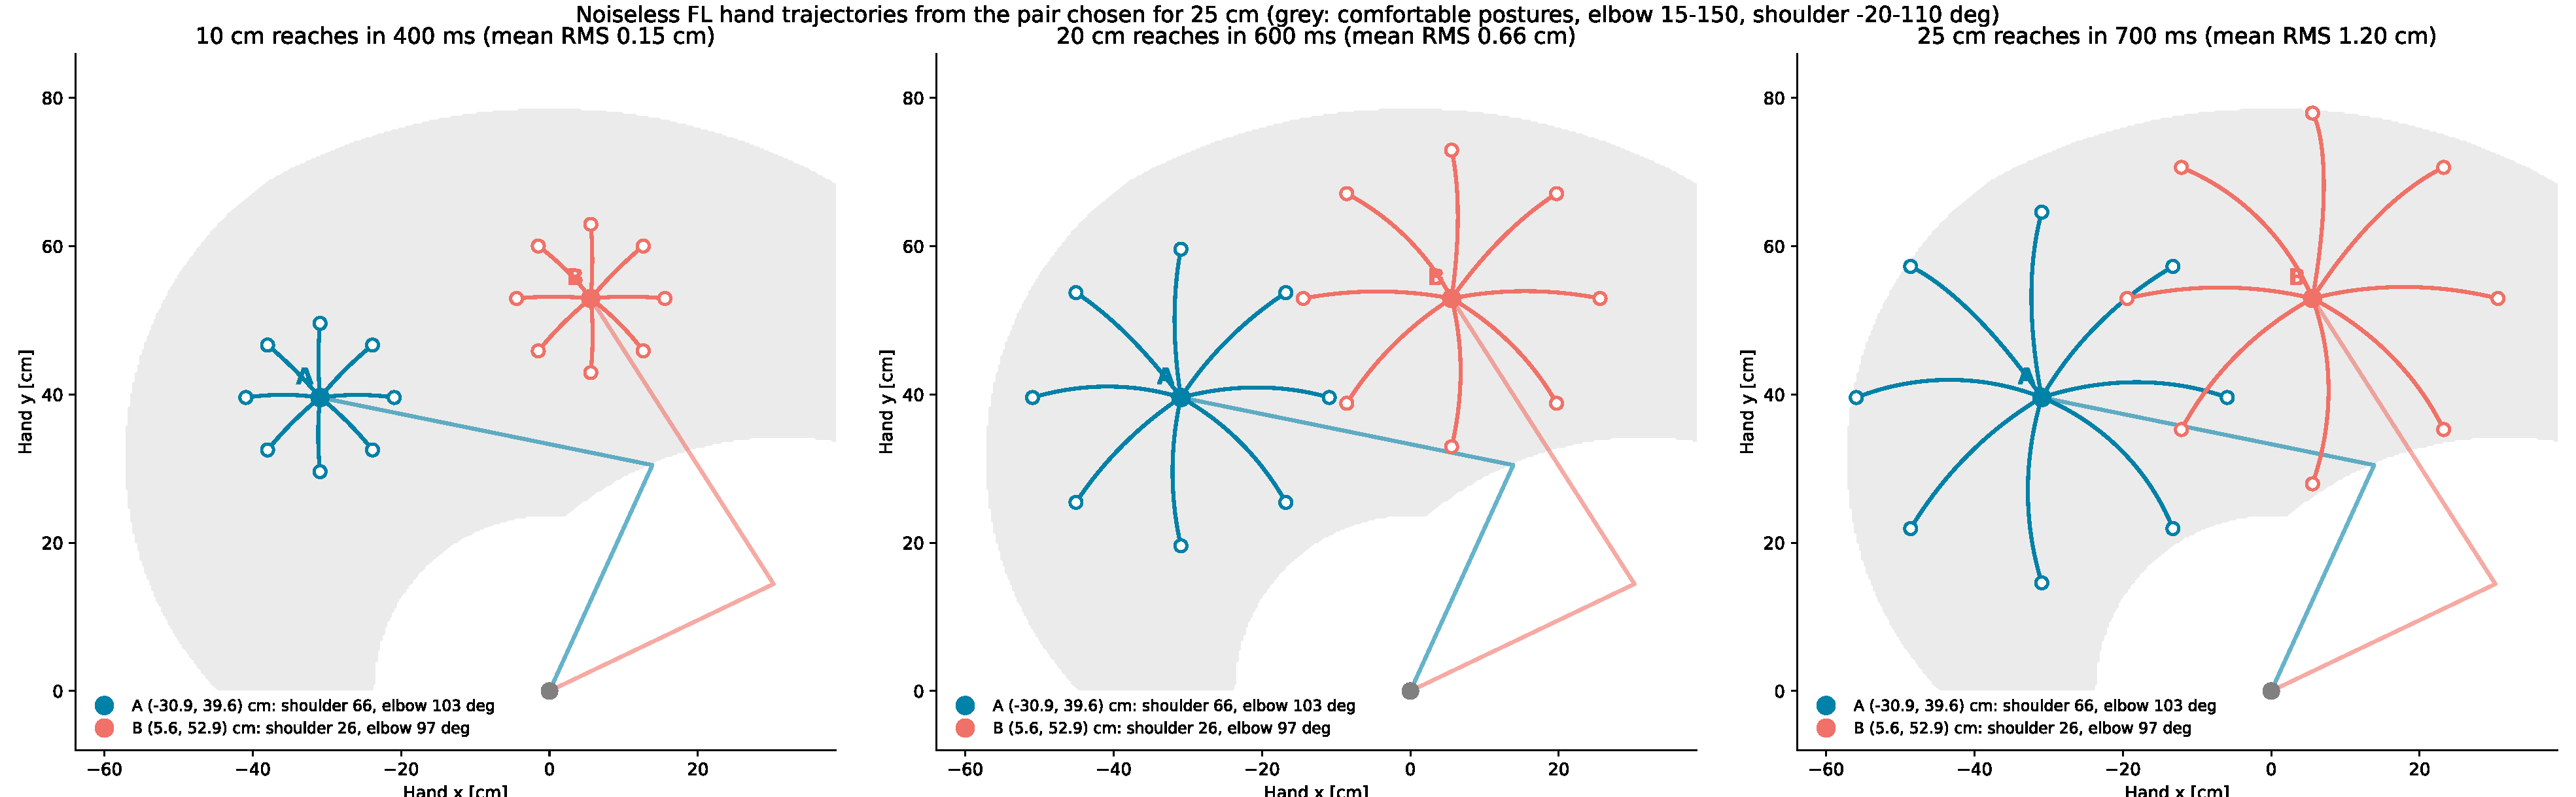
\includegraphics[width=\linewidth]{ChosenStarts_trajectories_25cm}
  \vspace{0.4em}
  \begin{itemize}\small
    \item Parmi les départs dont la posture et les 8 cibles sont confortables, on garde
          la paire dont les trajectoires FL (sans bruit) diffèrent le plus (RMS moyen sur 8 directions).
    \end{itemize}
\end{frame}

% =========================================================================
\section{WP1 -- Paramètres musculaires humains}

\begin{frame}{Centre-out 15\,cm / 400\,ms : LQG vs iLQG}
  \begin{columns}[c]
    \begin{column}{0.48\textwidth}
      \centering
      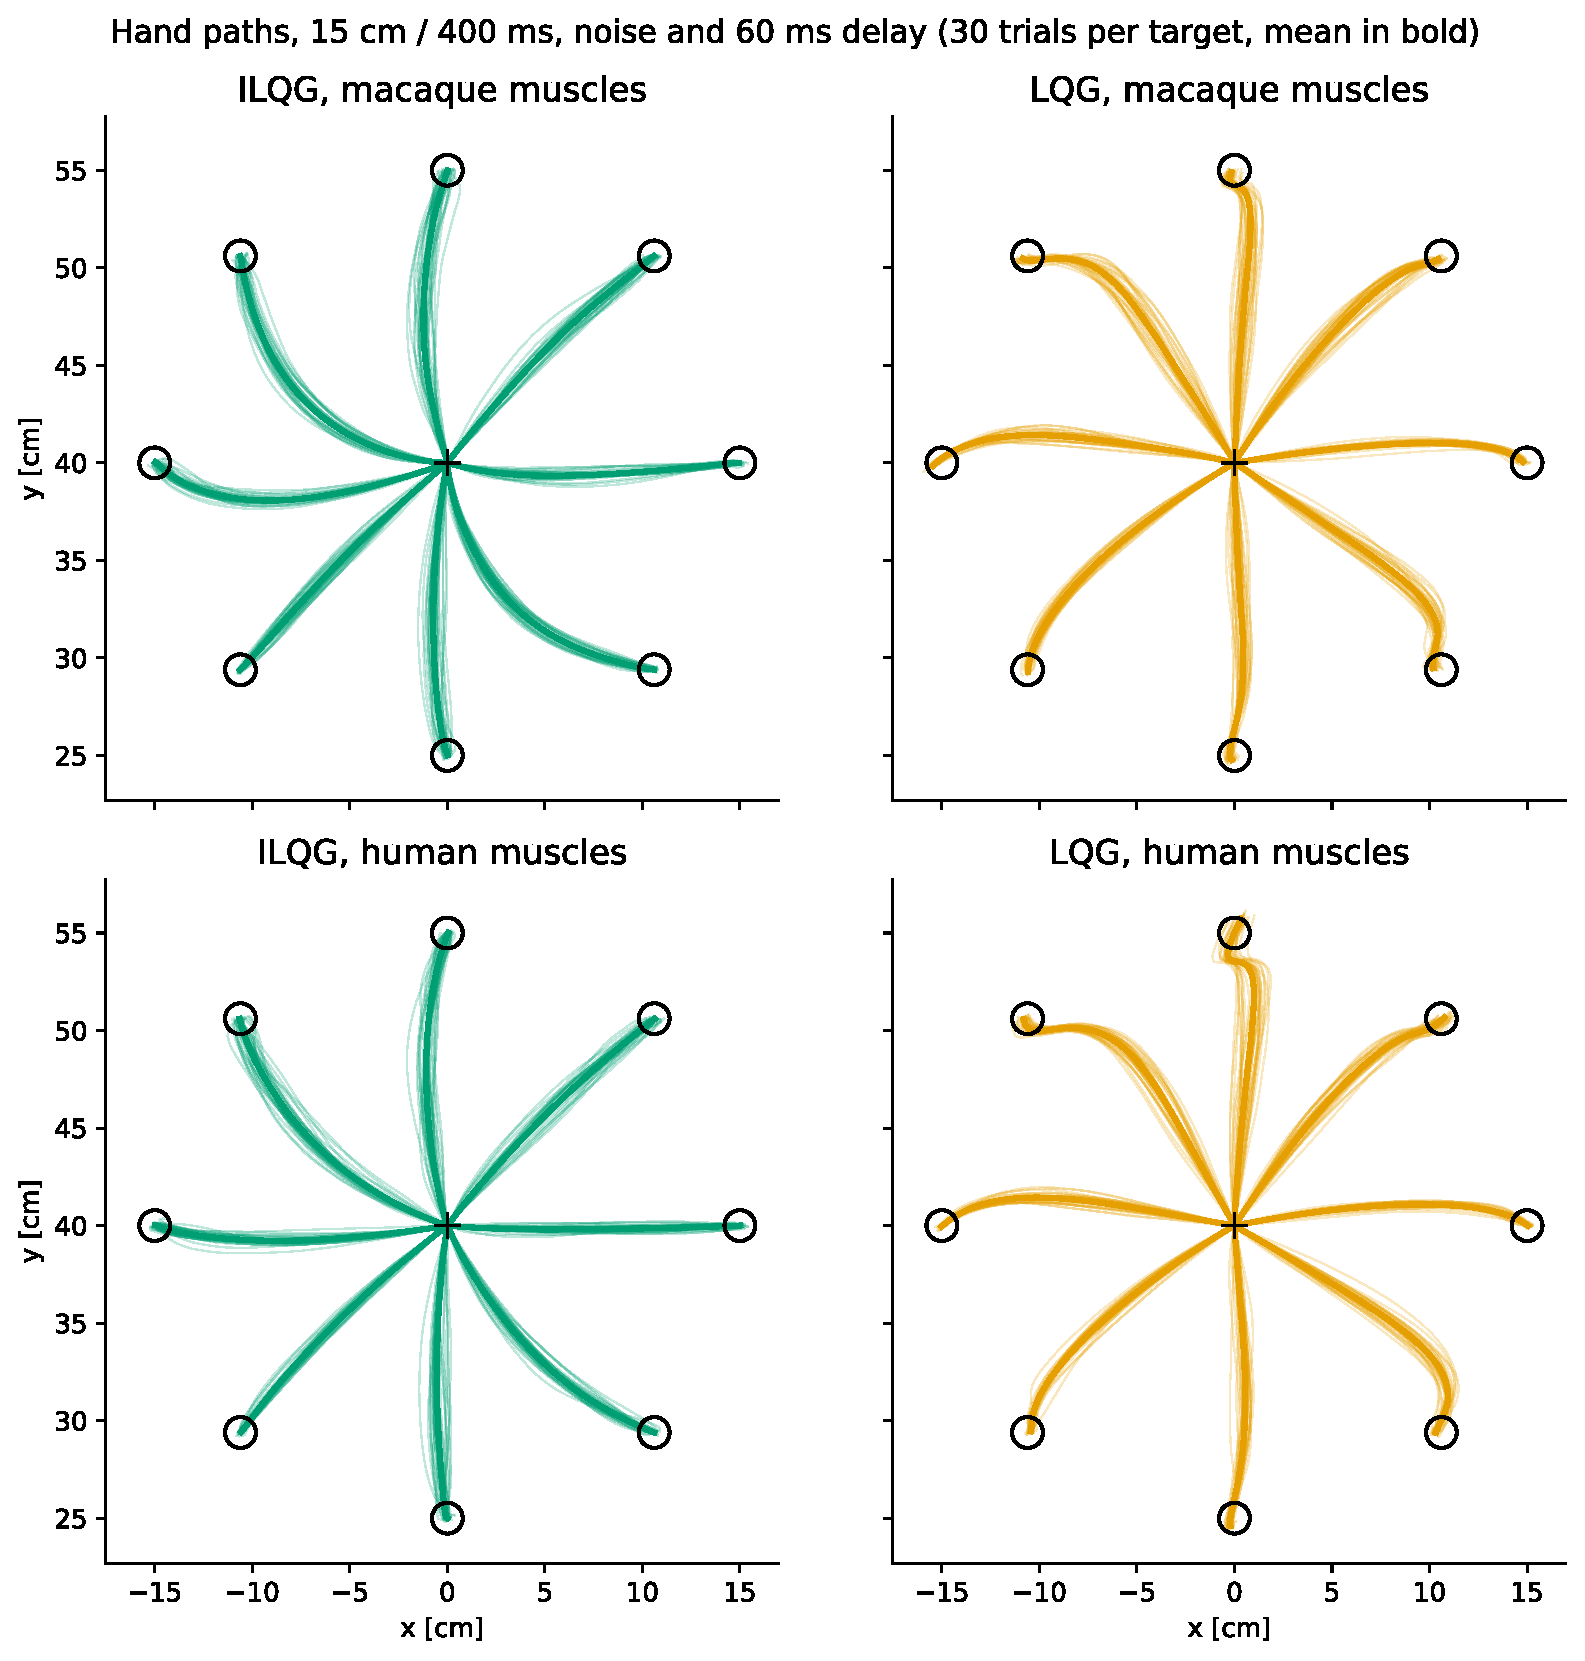
\includegraphics[height=0.82\textheight]{trajectories_15cm_400ms}
    \end{column}
    \begin{column}{0.48\textwidth}
      \small
      \begin{itemize}
        \item Comparaison avec des données musculaires issues de MotorNet.
        \end{itemize}
    \end{column}
  \end{columns}
\end{frame}

\begin{frame}{Coûts : iLQG nettement moins cher, surtout avec les muscles humains}
  \centering
  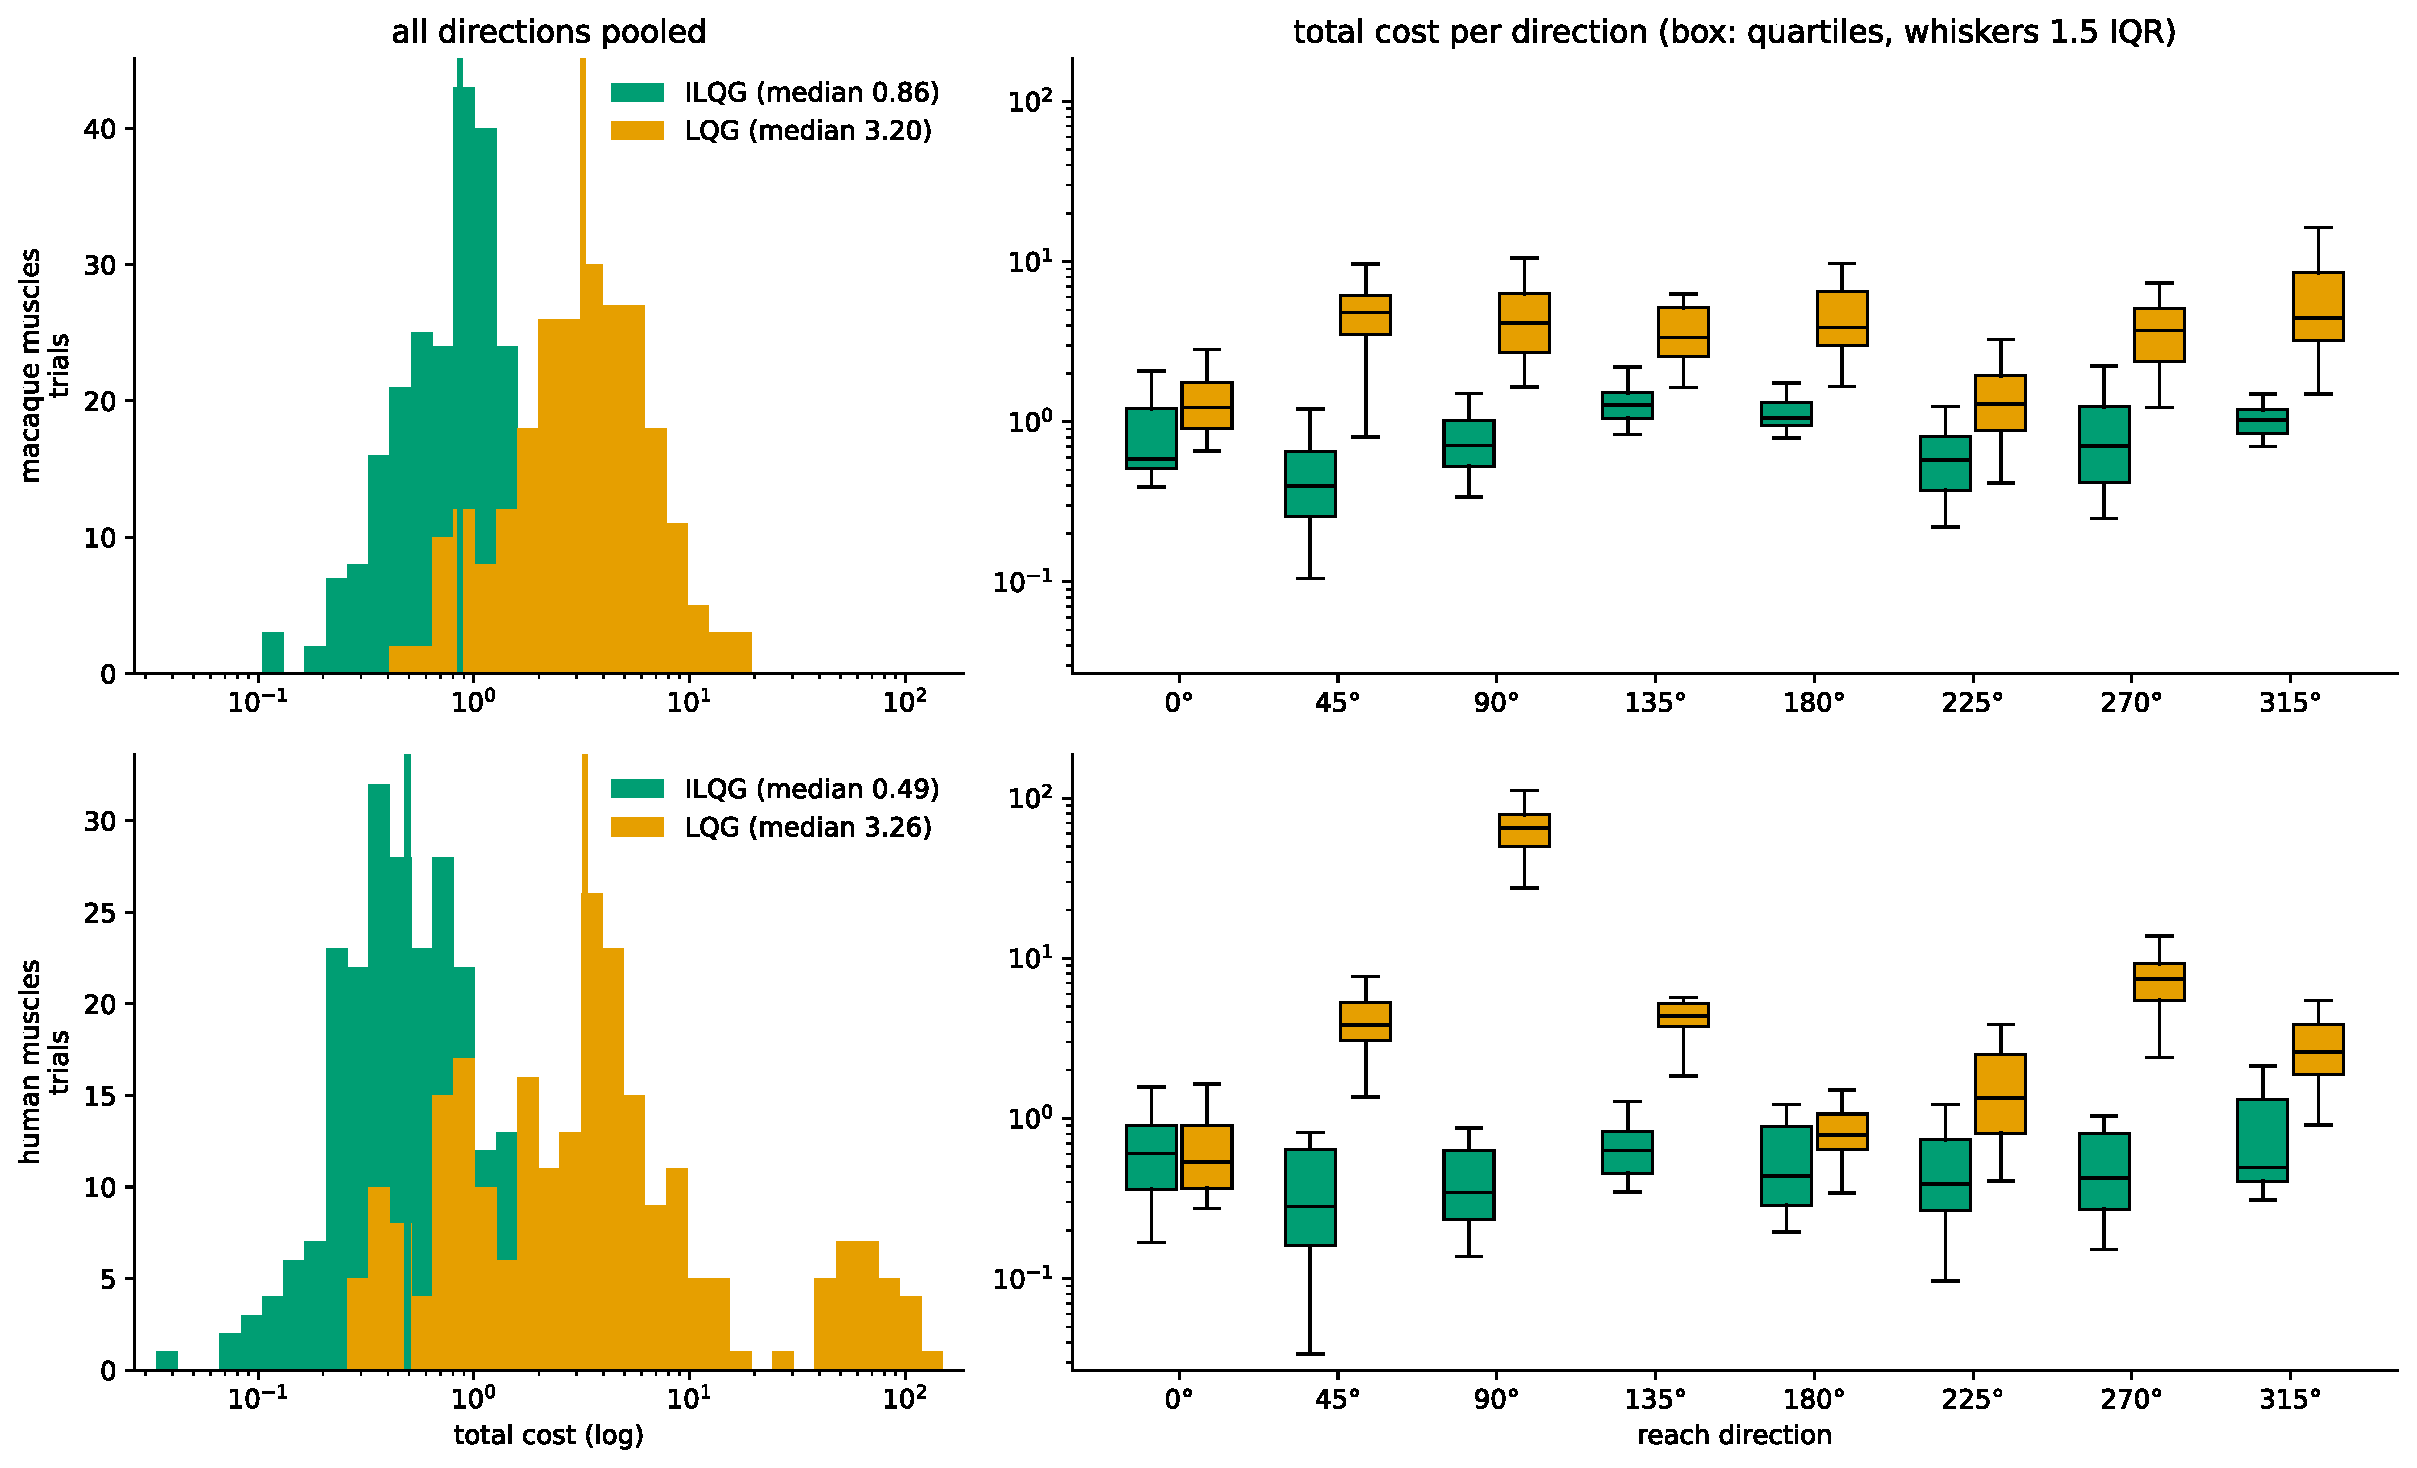
\includegraphics[width=0.68\linewidth]{cost_distributions_15cm_400ms}
  \vspace{0.3em}
  \end{frame}

\begin{frame}{Grands mouvements (600\,ms) : iLQG, macaque vs humain}
  \centering
  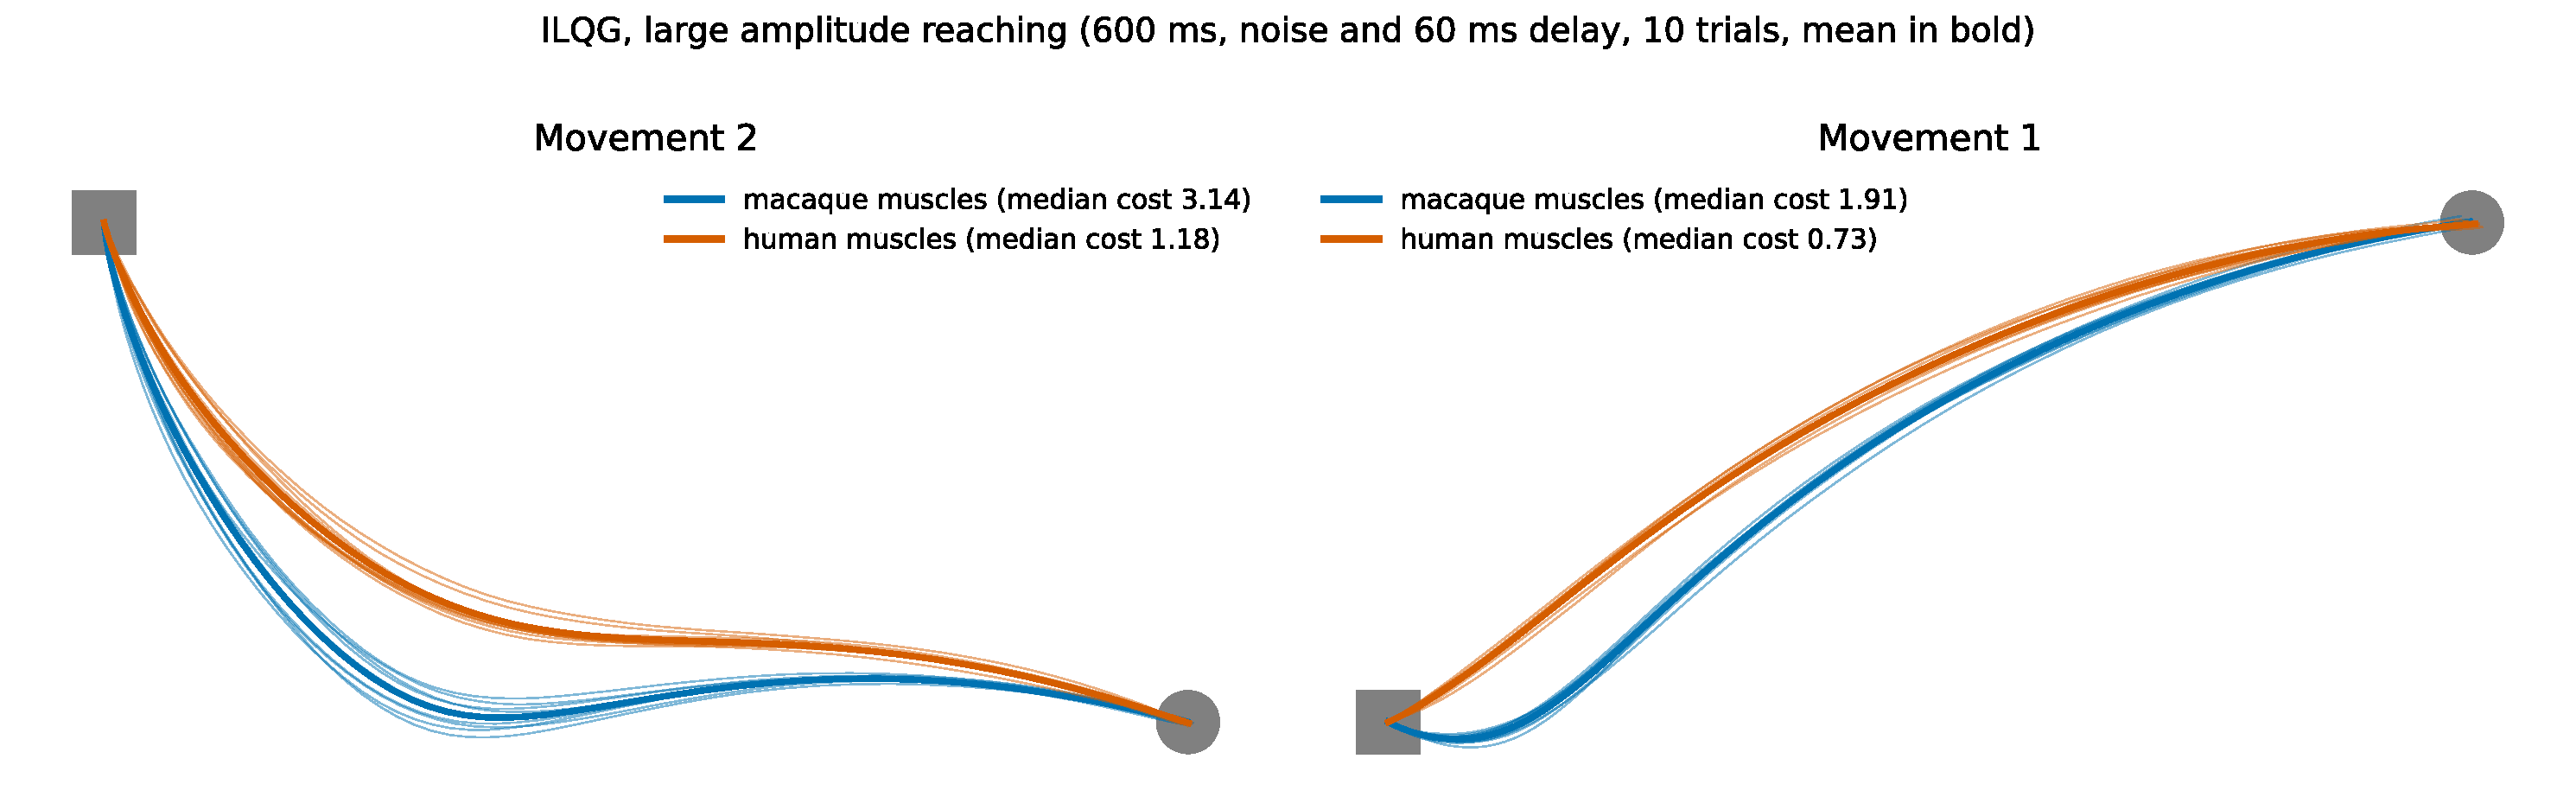
\includegraphics[width=\linewidth]{long_move_ilqg_macaque_vs_human}
\end{frame}

% =========================================================================
\section{WP3 -- Lillicrap \& Scott (2013), Fig.~5}

\begin{frame}{Construction : six échelons biomécaniques}
  \small
  \begin{columns}[t]
    \begin{column}{0.40\textwidth}
      \textbf{Commun}
      \begin{itemize}\footnotesize
        \item Réseau $\dot r = W r + u$, $N=100$, $W=(gX-I)/\tau_r$, $g=0.8$, $\tau_r=20$\,ms.
        \item $u$ optimisé par iLQG, lecture fixe aléatoire $W_{out}$.
        \item Bras macaque (Cheng \& Scott 2000), 16 cibles, 6\,cm en 0.4\,s.
        \item 20 couples (réseau, $W_{out}$), identiques à tous les échelons.
        \item Axe : $\theta = \tfrac12 \arg\big(\tfrac1n \sum_i e^{\,\mathrm{i}\,2\varphi_i}\big)$
              sur les PD des unités.
      \end{itemize}
    \end{column}
    \begin{column}{0.56\textwidth}
      \textbf{Échelons}\\[0.3em]
      \footnotesize
      \begin{tabular}{@{}cl@{}}
        \toprule
        1 & masse ponctuelle 2D, forces cartésiennes \\
        2 & + géométrie (bras 2 articulations, inertie diagonale) \\
        3 & + dynamique intersegmentaire (couplage, Coriolis) \\
        4 & + 4 muscles monoarticulaires (tirent seulement) \\
        5 & + 2 muscles biarticulaires \\
        6 & + mécanique musculaire F-L/V (Brown et al.\ 1999) \\
        \bottomrule
      \end{tabular}
    \end{column}
  \end{columns}
\end{frame}

\begin{frame}{Viscosité faible (Todorov) : l'axe suit la référence}
  \centering
  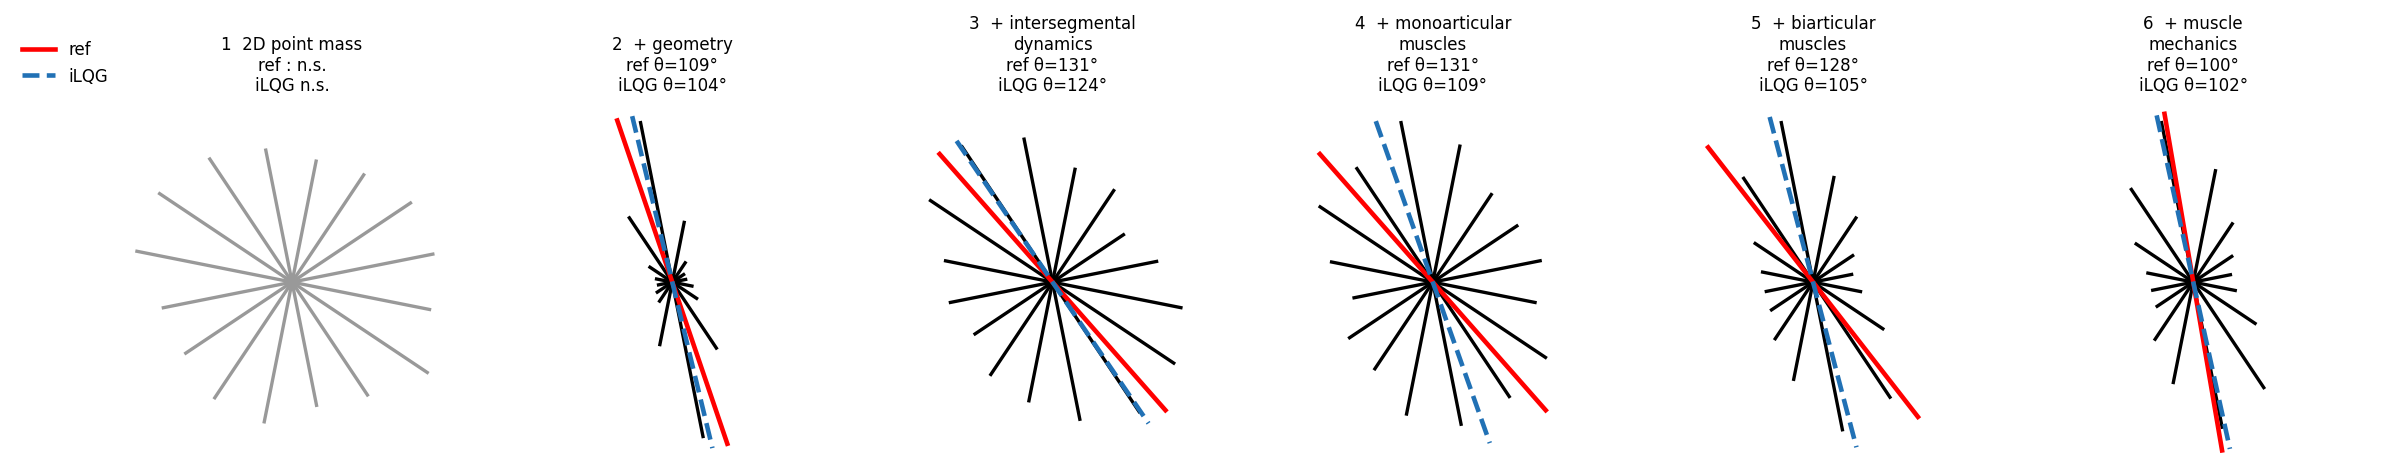
\includegraphics[width=\linewidth]{fig5_overlay_6cm_040s_macaque_todorov_cheng_scott}
  \vspace{0.4em}
  \begin{itemize}\small
    \item $B = \begin{bmatrix}0.05 & 0.025\\ 0.025 & 0.05\end{bmatrix}$\,N\,m\,s/rad.
          Rouge : axe de L\&S ; bleu pointillé : notre iLQG.
    \end{itemize}
\end{frame}

\begin{frame}{Viscosité forte (Kalidindi) : l'axe ne bouge plus}
  \centering
  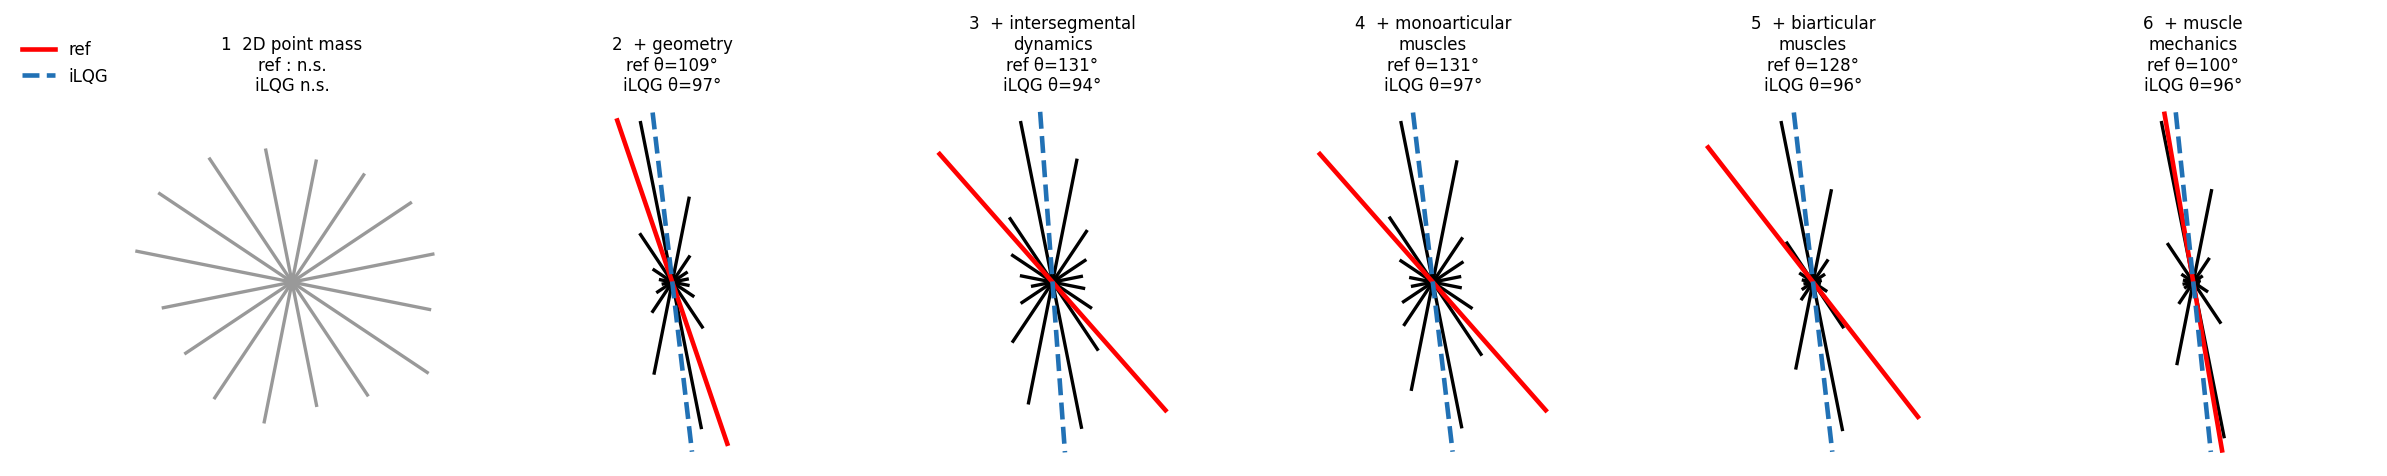
\includegraphics[width=\linewidth]{fig5_overlay_6cm_040s_macaque_kalidindi_cheng_scott}
  \vspace{0.4em}
  \begin{itemize}\small
     \item Seul l'échelon 6 reste proche de la référence (96/100).
  \end{itemize}
\end{frame}
\end{document}
